%%%%%%%%%%%%%%%%%%%%%%%%%%%%%%%%%%%%%%%%%%%%%%%%%%%%%%%%%%%%%%%%%%%%%%%%%%%%%%%
%
% REPORT  DESCRIPTION:
%   A concise description of the main concepts of the capstone.
%
% RESEARCH:
%   A list of research activities which led to this capstone.
%
% EXPERIMENTS:
%   A list of the experiments performed which supported the research.
%
%%%%%%%%%%%%%%%%%%%%%%%%%%%%%%%%%%%%%%%%%%%%%%%%%%%%%%%%%%%%%%%%%%%%%%%%%%%%%%%
\documentclass[12pt,american]{report}
\usepackage{rit-cs-capstone}
%%%%%%%%%%%%%%%%%%%%%%%%%%%%%%%%%%%%%%%%%%%%%%%%%%%%%%%%%%%%%%%%%%%%%%%%%%%%%%%
%   The following packages are all optional and depend on the specifics of what
% is contained in the capstone.  There is no harm in leaving them in.
%%%%%%%%%%%%%%%%%%%%%%%%%%%%%%%%%%%%%%%%%%%%%%%%%%%%%%%%%%%%%%%%%%%%%%%%%%%%%%%
\usepackage{subfigure}
\usepackage[refpages]{gloss}
\usepackage{babel}
\usepackage{times}
\usepackage{graphicx}
\usepackage{amssymb}
\usepackage{lscape}
\usepackage{verbatim}
\usepackage{enumerate}
\usepackage{afterpage}
\usepackage{listings}
\usepackage{float}
\usepackage{url}
\usepackage{upquote}

\lstset{numbers=left,
 frame=single,
 columns=fullflexible,
 basicstyle=\small\ttfamily,
 numberstyle=\tiny,
 showstringspaces=false,
 captionpos=b,}
%%%%%%%%%%%%%%%%%%%%%%%%%%%%%%%%%%%%%%%%%%%%%%%%%%%%%%%%%%%%%%%%%%%%%%%%%%%%%%%
%   Mark the document as 'draft' with a date. Be sure to comment this out for
% the final version.
%\usepackage{draftwatermark}
%\SetWatermarkLightness{0.9}
%\SetWatermarkText{DRAFT}
%\SetWatermarkScale{1}

%\usepackage{watermark}
%\watermark{\hspace{-0.3in} \textbf{DRAFT} \hspace{2.0in} \textbf{\today}}

%\usepackage{draftcopy}
%%%%%%%%%%%%%%%%%%%%%%%%%%%%%%%%%%%%%%%%%%%%%%%%%%%%%%%%%%%%%%%%%%%%%%%%%%%%%%%

\makegloss

\begin{document}
%%%%%%%%%%%%%%%%%%%%%%%%%%%%%%%%%%%%%%%%%%%%%%%%%%%%%%%%%%%%%%%%%%%%%%%%%%%%%%%
% Title page
% The \title{} can contain line breaks as appropriate...
\title{\vspace{-0.20in}Buffalo: An Aspect Oriented Programming Framework for C\#}
% The \titleline{} must have no line breaks in it.
\titleline{Buffalo: An Aspect Oriented Programming Framework for C\#}
% This is not a thesis but a project
\MSprojecttrue
% This date is really not used (unless \grantdate{}{} is blank)
\date{February 2013}
%%%%%%%%%%%%%%%%%%%%%%%%%%%%%%%%%%%%%%%%%%%%%%%%%%%%%%%%%%%%%%%%%%%%%%%%%%%%%%%

%%%%%%%%%%%%%%%%%%%%%%%%%%%%%%%%%%%%%%%%%%%%%%%%%%%%%%%%%%%%%%%%%%%%%%%%%%%%%%%
% Author information page
% The \author{} should be exactly the same as your diploma
\author{Wei Liao}
%%%%%%%%%%%%%%%%%%%%%%%%%%%%%%%%%%%%%%%%%%%%%%%%%%%%%%%%%%%%%%%%%%%%%%%%%%%%%%%

%%%%%%%%%%%%%%%%%%%%%%%%%%%%%%%%%%%%%%%%%%%%%%%%%%%%%%%%%%%%%%%%%%%%%%%%%%%%%%%
% The following information is for the signature page.
% Note that the definition for principal adviser uses two fields.
% This was needed so that the adviser's name could be placed on the
% abstract page without his/her title.
\committeechair{Prof. James E. Heliotis}{Professor}
\reader{Prof. Matthew Fluet\\ Assistant Professor}
\observer{Prof. Fereydoun Kazemian\\ Associate Professor}
%%%%%%%%%%%%%%%%%%%%%%%%%%%%%%%%%%%%%%%%%%%%%%%%%%%%%%%%%%%%%%%%%%%%%%%%%%%%%%%

%%%%%%%%%%%%%%%%%%%%%%%%%%%%%%%%%%%%%%%%%%%%%%%%%%%%%%%%%%%%%%%%%%%%%%%%%%%%%%%
% This is the expected date that the committee will sign your Capstone.
\grantdate{April}{2013}
%%%%%%%%%%%%%%%%%%%%%%%%%%%%%%%%%%%%%%%%%%%%%%%%%%%%%%%%%%%%%%%%%%%%%%%%%%%%%%%

%%%%%%%%%%%%%%%%%%%%%%%%%%%%%%%%%%%%%%%%%%%%%%%%%%%%%%%%%%%%%%%%%%%%%%%%%%%%%%%
% If you want to copyright your capstone remove the line below.
\copyrightfalse% True by default
% The year of the copyright; usually same as the date the committee will
% sign the \item{} . This won't be printed if \copyrightfalse
\copyrightyear{2013}
%%%%%%%%%%%%%%%%%%%%%%%%%%%%%%%%%%%%%%%%%%%%%%%%%%%%%%%%%%%%%%%%%%%%%%%%%%%%%%%

%%%%%%%%%%%%%%%%%%%%%%%%%%%%%%%%%%%%%%%%%%%%%%%%%%%%%%%%%%%%%%%%%%%%%%%%%%%%%%%
% This causes all front matter to be set.
\beforepreface%
%%%%%%%%%%%%%%%%%%%%%%%%%%%%%%%%%%%%%%%%%%%%%%%%%%%%%%%%%%%%%%%%%%%%%%%%%%%%%%%

%%%%%%%%%%%%%%%%%%%%%%%%%%%%%%%%%%%%%%%%%%%%%%%%%%%%%%%%%%%%%%%%%%%%%%%%%%%%%%%
% The dedication - if you choose to include one.
% It should be vertically centered in the page. Since the style format doesn't 
% do it for you automatically, you can use the following technique.
\prefacesection{Dedication}
\vfill
\begin{center}
To Jackson and Evan
\end{center}
\vfill
%%%%%%%%%%%%%%%%%%%%%%%%%%%%%%%%%%%%%%%%%%%%%%%%%%%%%%%%%%%%%%%%%%%%%%%%%%%%%%%

%%%%%%%%%%%%%%%%%%%%%%%%%%%%%%%%%%%%%%%%%%%%%%%%%%%%%%%%%%%%%%%%%%%%%%%%%%%%%%%
% The acknowledgements page - if you choose to include one. 
% As in the dedication, it should be centered vertically in the page.
%
\prefacesection{Acknowledgments}
%\vfill
%\begin{center}
I am grateful for my adviser Prof. Heliotis, whose insightful advice, guidance and support from the beginning not only enabled me to complete the project on time, but also led me to a better understanding of the subject area.

I am also grateful for Prof. Fluet and Prof. Kazemian for their invaluable feed backs.

Last but not the least, I want to thank my wife Michelle, for all the support and encouragement during my years at school.
%\end{center}
%\vfill
%%%%%%%%%%%%%%%%%%%%%%%%%%%%%%%%%%%%%%%%%%%%%%%%%%%%%%%%%%%%%%%%%%%%%%%%%%%%%%%

%%%%%%%%%%%%%%%%%%%%%%%%%%%%%%%%%%%%%%%%%%%%%%%%%%%%%%%%%%%%%%%%%%%%%%%%%%%%%%%
%%  Collection of useful abbreviations.
\newcommand{\etc} {\emph{etc.\/}}
\newcommand{\etal}{\emph{et~al.\/}}
\newcommand{\eg}  {\emph{e.g.\/}}
\newcommand{\ie}  {\emph{i.e.\/}}
%%%%%%%%%%%%%%%%%%%%%%%%%%%%%%%%%%%%%%%%%%%%%%%%%%%%%%%%%%%%%%%%%%%%%%%%%%%%%%%


%%%%%%%%%%%%%%%%%%%%%%%%%%%%%%%%%%%%%%%%%%%%%%%%%%%%%%%%%%%%%%%%%%%%%%%%%%%%%%%
% Abstract
\begin{abstractpage}
Aspect Oriented Programming (AOP) is a paradigm that let programmer isolate and separate crosscutting concerns from their programs. The concept has not been widely adopted by modern languages; support in tooling such as Integrated Development Environment (IDE) is also rare. In this project I designed and implemented Buffalo, an AOP framework to provide this capability for the .NET platform.

Buffalo performs MSIL instruction set modification according to the aspects written by developer, with the help of the Mono Cecil library. Buffalo is .NET attribute based, which mean developers with existing .NET skills will have little or no learning curve to get started. Buffalo will help increase developer productivity in many area such as unhandled exception catching, tracing and logging, and many other areas.
\end{abstractpage}

%%%%%%%%%%%%%%%%%%%%%%%%%%%%%%%%%%%%%%%%%%%%%%%%%%%%%%%%%%%%%%%%%%%%%%%%%%%%%%%

%%%%%%%%%%%%%%%%%%%%%%%%%%%%%%%%%%%%%%%%%%%%%%%%%%%%%%%%%%%%%%%%%%%%%%%%%%%%%%%
% Uncomment the line below if you don't want a list of tables to be printed.
% \tablespagefalse

% Uncomment the line below if you don't want a list of figures to be printed.
% \figurespagefalse

% \afterpreface generates the table of contents, list of tables (optional),
% and list of figures (optional).
\afterpreface%
%%%%%%%%%%%%%%%%%%%%%%%%%%%%%%%%%%%%%%%%%%%%%%%%%%%%%%%%%%%%%%%%%%%%%%%%%%%%%%%

%We don't need a glossary so comment it out.
%\printgloss{Glossary}

%%%%%%%%%%%%%%%%%%%%%%%%%%%%%%%%%%%%%%%%%%%%%%%%%%%%%%%%%%%%%%%%%%%%%%%%%%%%%%%
% This is where the main body of the capstone report starts
\body%

\chapter{Introduction}

%% Obviously you need to delete these lines when you have written up your text


\begin{itemize}
\item{} Background: should be sufficient for the reader understand the rest of the report, but 
perhaps not too long to put the reader to sleep.
\item{} Basic problem definition and motivation
\item{} Approaches used to solve the problem (related work)
\item{} Hypothesis: what you think the problem is and how your solution 
approach will address the problem
\item{} Roadmap: how the rest of your report is laid out 
\end{itemize}

And yes, this is how you cite a book by Silberschatz~\cite{Silberschatz05-text} or a paper by Dumont~\cite{Dumont2007-robots}.

And here are examples of how to include figures and tables in the text. Please note that the captions go below for figures and above for tables.


\begin{figure}[ht]
\begin{center}

\includegraphics[width=3.0in]{cs-logo.jpg}
\end{center}
\caption{The CS Logo is Above}
\label{fig:lab}
\end{figure}


\begin{table}[h]
\caption{The Dog Table is Below}
  \begin{tabular}{ | l | c | r | }
    \hline
    tag & breed & age \\
    \hline \hline
    13 & Fido & 2 \\
    \hline
    14 & Fifi & 4 \\
    \hline
  \end{tabular}
\end{table}

For both tables and figures, the optional argument controls
placement as shown:
\begin{itemize}
  \item{} h is Here, i.e., the position in the text where the table environment appears.
  \item{} t is Top, i.e., the top of a text page.
  \item{} b is Bottom, i.e., at the bottom of a text page.
  \item{} p is Page of floats, i.e., on a separate float page,
    which is a page containing no text, only floats.
\end{itemize}

Anyway, you can find some easy tutorials on \LaTeX{}.
\chapter{Design}

\section{Compiler Support}

There are several broad approaches to implementing an AOP framework. The ideal approach would be to extend the compiler of the target language to provide built-in support, thus making AOP the first class citizen. However there are very few languages out there that take this approach, among the few are Delphi Prism~\cite{delphi_prism2010} and AspectJ~\cite{aspectj_faq, aspectj_text}. 

Microsoft is currently in the "wait and see" mode regarding support of AOP development in the C\# compiler~\cite{hejlsberg}. Alternative compiler such as Mono C\#~\cite{monocsharp} is open source, so technically anyone can build AOP support into it. While that would have been a fun challenge, that would have been a fairly big undertaking, and there is concern that the project might not be finished in the time frame wanted.

That leaves framework support as the other viable option. There are several implementation techniques to provide AOP capabilities~\cite{aopcs, postsharp, aspectcs} via framework.

\section{Run-time Interception}

Early on the implementation approaches were narrowed down to between Run-time Interception and Compile Time Weaving. As its name suggested, run-time interception operates while the program is in execution. It uses the proxy pattern where client communicate with the target object via a proxy, and aspects are injected to the proxy. This enables run-time behavior of the program to be modified. Figure~\ref{proxy_model} illustrates this process.

\begin{figure}[H]
  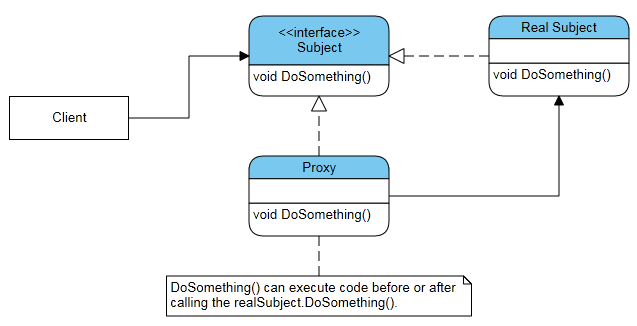
\includegraphics[scale=1.0]{Proxy2.PNG}
  \centering
  \caption{AOP Framework Using Proxy Pattern\label{proxy_model}}
\end{figure}

New functionality can be “added” to the target object via the proxy. The disadvantage of this approach is that it involves the generation of proxy object at run-time. The run-time performance of the application will be impacted as the result. It is also restricting in that both target object and the proxy must implement a common interface for this to work, and that only virtual methods are exposed for interception.

From the end user's perspective, to use it the developer usually have to provide some type of mapping between the target object and the proxy via a configuration file so the actual proxy generation can occur. This approach although is easier to implement, but not as easy and friendly to use. Buffalo is not taking this approach mainly because one of the goal is to be flexible and simple to use.

\section{Post Compilation Weaving}

The approach Buffalo takes is Post Compilation Weaving. The idea is that after compilation of the source code, the framework takes over and disassembles the assembly. Buffalo then weaves in the defined aspect code to all targeted methods. This approach is more difficult to implement as it involves modifying the underlying assembly by changing Common Intermediate Language (CIL) instructions~\cite{rewrite_msil}. But the advantage is that no run-time performance of proxy generation will be needed. 

Since injection happens post-compilation, the whole process can be integrated into the MS-Build system to have the weaving invoked automatically if needed. This will further reduce the steps needed from the developer.

Figure~\ref{buffalo_model} shows an overview of the compilation process and where Buffalo will fit in.

\begin{figure}[H]
  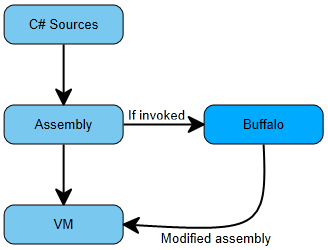
\includegraphics[scale=1.0]{BuffaloOverview.PNG}
  \centering
  \caption{Buffalo Model\label{buffalo_model}}
\end{figure}

\section{A Buffalo Aspect}

When performing post compilation weaving, Buffalo has to be able to discover what aspect is applied to what methods in an assembly. In order to achieve that, the target assembly has to carry some identifying meta-data.

A given .NET assembly already carries a great deal of such meta-data for various purpose. .NET has the System.Attribute type that exists primarily for the purpose of inserting meta-data into the assembly during compilation. When the source code is compiled, it is converted into CIL~\cite{msil_text} and put inside a portable executable (PE) file, with the meta-data generated by the compiler. 

Buffalo takes advantage of this characteristic in two phases.
\begin{enumerate}
	\item An aspect defined in Buffalo will be in the form of an attribute, by sub-classing System.Attribute. It can contain any valid .NET code. But specifically an aspect needs to override various predefined methods in order to do something useful. The next section will discuss the relationship between various aspect types.
	\item After compilation, the assembly will now contain the meta-data about the aspect. Buffalo can inspect the assembly for the information, and perform CIL code injection accordingly.
\end{enumerate}

In other word, a Buffalo aspect is a .NET attribute in disguise.

\section{MethodBoundaryAspect}
What functionality does Buffalo support? What type of weaving does it do? For inspiration existing works such as AspectJ~\cite{aspectj_faq} and PostSharp~\cite{postsharp} were studied. Specifically Buffalo will intercept the various point of an executing method. Those points are namely: before a method executes; after a method executes; whether or not the method executed successfully without error; or whether the method throws an exception any point during the execution. These various points of interception are grouped into the MethodBoundaryAspect.

MethodBoundaryAspect can be cleanly mapped to the try-catch-finally statements of the .NET languages. As far as the runtime is concern~\cite{ecma334, ecma335}, try-catch can be used liberally without serious performance degradation. For example, a simple method shown in Figure~\ref{samplefunction}:

\begin{lstlisting}[caption={Sample function}, label=samplefunction]
public void SomeFunction () {
   //Perform some action...
}
\end{lstlisting}

The above can be transformed by Buffalo into something shown in Figure~\ref{sampletcf}. This clearly captures the spirit of the MethodBoundaryAspect. Regardless of whether the source already contain its own try-catch, or try-catch-finally blocks, the body of the method will be wrapped inside of a new try-catch-finally block by Buffalo.

\begin{lstlisting}[caption={Sample try-catch-finally}, label=sampletcf]
public void SomeFunction () {
   try {
       OnBefore();
       //Perform some action
       OnSuccess();
   }
   catch (Exception e) {
       OnException(e);
   }
   finally {
       OnAfter();
   }
}
\end{lstlisting}

Transformed method in Figure~\ref{sampletcf} still does what the original method intends to do, only now at various point execution are being intercepted to provide more functionality. 

\section{MethodAroundAspect}
Another type of aspect that Buffalo supports is the MethodAroundAspect. Rather than intercepting various execution points of a method, the method can be completely replaced by another method defined in an aspect, while preserving the option to call back into the original method if necessary.

At first glance MethodAroundAspect sounds straightforward to do, but it turns out to be much more involved than the MethodBoundaryAspect.

Since the option to call back into the original method is preserved, it is critical that under no circumstance should the original method be modified. If the method body instructions are simply overridden with that of the replacement, the call back to the original method will be meaningless since the method is now changed. The original method must be intact for the call back to happen.

To get around this obstacle, whenever Buffalo encounters the MethodAroundAspect applied to a method, it dynamically generates a replacement method in CIL with the same method signature as the original.

The body of this replacement method is also completely different than the original. It instantiates the aspect and makes call to the Invoke() method, which is the actual code that will be ran as a replacement. 

Inside the Invoke method, developer can make a call back to the original method via a call to the Proceed() method. Then throughout the program, for any calls made to the original method, Buffalo would change them to call the replacement method instead. This is illustrated in figure~\ref{around_overview}.

\begin{figure}[H]
  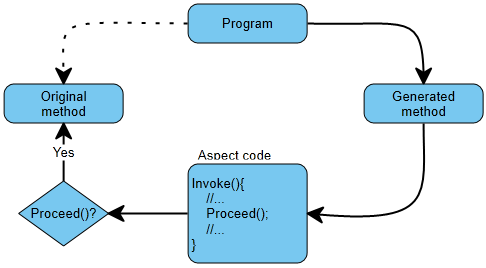
\includegraphics[scale=1.0]{AroundOverview.PNG}
  \centering
  \caption{Overview of MethodAroundAspect\label{around_overview}}
\end{figure}

The dotted line from Program to the Original method indicates that once the MethodAroundAspect is applied to it, from the perspective of CIL the program cannot directly access that method any more. Access to the original method now has to come from inside the aspect. Also note that the original method is not changed at any given time.

\chapter{Implementation}

\section{How to Apply an Aspect}

Since an aspect is really a .NET attribute, it can be used just like any other attribute. But code annotated with an aspect is special in that it can be understood only by Buffalo.

A Buffalo aspect can be applied on three levels, with the following characteristics:

\begin{enumerate}
  \item Method - apply the aspect to an individual method.
  \item Class - if aspect is applied to a class, all public methods including the public properties automatically get applied.
  \item Assembly - if aspect is applied to an assembly, \#2 will apply but for all the public classes within the assembly.
\end{enumerate}

An exception to the above rule is the MethodAroundAspect, where it can only be applied on a method level, as will be shown later on.

All aspects have a property named AttributeExclude, if set to true then the annotated target will not be included in the weaving. This exclusion can happen on any levels. For example, if a method contains this annotation [SampleAspect(AttributeExclude=true)], the method will be skipped for the SampleAspect during the weaving process.

No matter how the aspect is applied, ultimately it will result in a list of the methods that are annotated. This simply mean if the aspect is applied to a single method, that method is the only one that will get CIL modified. If the aspect is applied on the whole assembly, then all public methods will be CIL modified.

To get the list of the eligible methods for CIL modification, Buffalo attempts various checking according to figure~\ref{logical_inclusion} to see if it should include a given method.

\begin{figure}[H]
  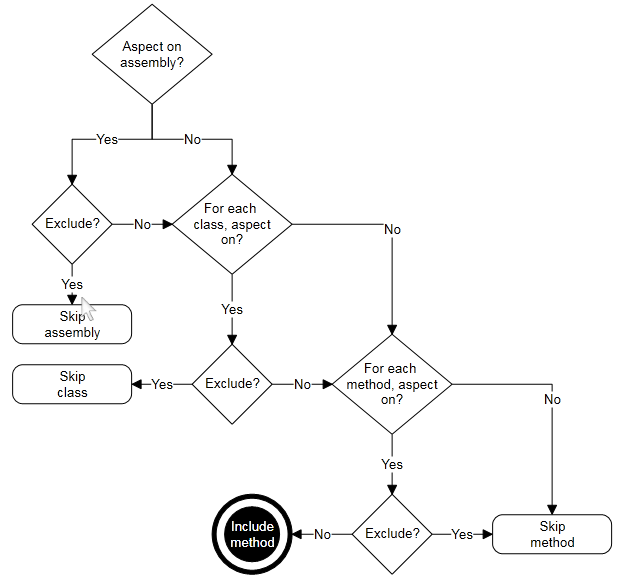
\includegraphics[scale=1.0]{AspectLogicalInclusion2.PNG}
  \centering
  \caption{Diagram for Finding Eligible Methods\label{logical_inclusion}}
\end{figure}

If no aspect is applied on the assembly, that does not necessarily mean no aspect is applied anywhere, the aspect might still be applied on any given class or method.

Buffalo first checks if an aspect is applied to the target, then check if it is set to be excluded. At the end it will end up with a list of methods that should be CIL modified.

\section{Aspect Interface}

Figure~\ref{uml01} shows the relationship of various aspect types in Buffalo. This is used by Buffalo to identify aspects during reflection.

\begin{figure}[H]
  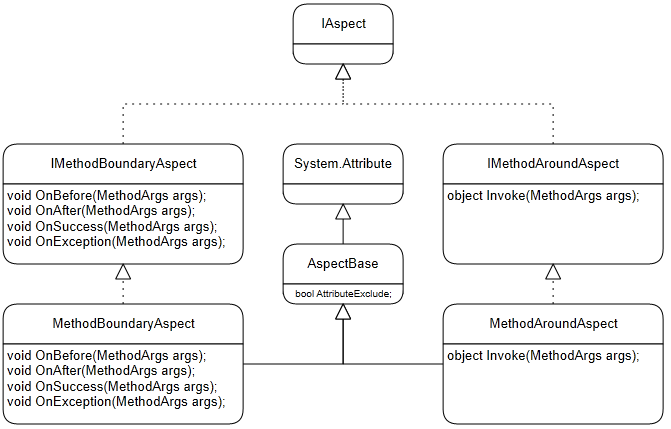
\includegraphics[scale=1.0]{Uml02.PNG}
  \centering
  \caption{Aspect Inheritance\label{uml01}}
\end{figure}

All aspects ultimately implements the IAspect interface, therefore it can be reasoned that for all the public types in an assembly, if it implements IAspect, then it must be an aspect itself.

Buffalo supports more than one aspect applied at any given level. This will allow developers more flexibility while developing multiple aspects and applying them as needed.

Furthermore, by default, an aspect will be automatically excluded from applying to itself. This is implemented to prevent stack overflow in some cases. Although argument can be made that an aspect should be able to be applied to a different aspect; that is not currently implemented in Buffalo.

Listing~\ref{aspectexample} shows how a simple aspect is created. It inherits MethodBoundaryAspect and overrides OnBefore and OnAfter.

\begin{lstlisting}[caption={Sample TraceAspect}, label=aspectexample]
using Buffalo;
using System;

public class TraceAspect : MethodBoundaryAspect
{
    public override void OnBefore(MethodArgs args)
    {
        Display("ENTERING", args);
    }

    public override void OnAfter(MethodArgs args)
    {
        Display("EXITING", args);
    }

    void Display(string title, MethodArgs args)
    {
        Console.WriteLine("{0} {1}", title, args.FullName);
        foreach (var p in args.Parameters)
        {
            Console.WriteLine("\t{0} ({1}) = {2}", 
			p.Name, p.Type, p.Value);
        }
    }
}
\end{lstlisting}

To use the aspect, simply apply it to a method, class or assembly. Once the code is compiled to produce an assembly, BuffaloAOP.exe can be invoked by passing it the path to the assembly. Buffalo will take over and weave in the aspect. This and more examples and details are provided in Appendix A.

\begin{lstlisting}[caption={Apply Aspect on Class Level}, label=helloaspect]
[TraceAspect]
public class Hello
{
	//...
}
\end{lstlisting}

\section{MethodArgs}

As mentioned above, when all is said and done, an aspect ultimately gets injected into each \textit{individual} method. When developing an aspect, meta-information about the target method can be accessed. This information is encapsulated via the MethodArgs object passed in as parameter to the aspect. Method name; its full method signature; return type and parameter list (including parameter name, type and value) are captured for each target method.

The parameter list capturing is especially of interest, it enables developer to peek inside the method that is executing at various point and inspect its parameter values. This will be useful in case such as exception handling, where it will be useful to actually see what the values were at the time of the exception. When using MethodAroundAspect, the parameter values can even be modified and pass back to the original method.

\section{Visual Studio Solution Structure}

Originally Buffalo was implemented as one executable; that includes the various aspects and the program that initiates the weaving. It was later on separated into two assemblies. One is a class library that contains the actual implementation. Another is a command line executable that calls into the class library to perform the weaving. This separation is necessary so developer can perform weaving from the command line or hook into MS-Build if necessary. 

To actually write the aspect, one only needs to reference the class library as underlined in figure~\ref{solutionexplorer}.

\begin{figure}[H]
  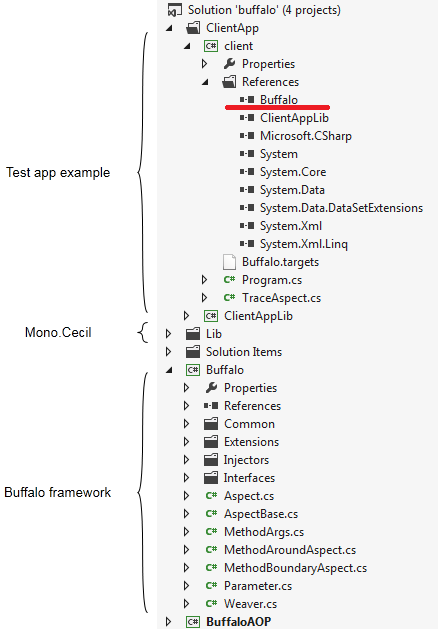
\includegraphics[scale=1.0]{SolutionExplorer3.PNG}
  \centering
  \caption{Solution Structure\label{solutionexplorer}}
\end{figure}

The client project shown above is a simple program included in the solution for testing.

\section{Implementation Overview}

The implementation begins by finding all eligible methods to be injected using the verifying process indicated in figure~\ref{logical_inclusion}. Each eligible method will have one or more aspects applied to it. The actual injection process will loop through each aspects for the eligible method and inject the necessary CIL instructions.

The CIL instructions modification is performed by using the open source Mono.Cecil library. Originally the System.Reflection APIs in the .NET Framework was favored, but it was later determined that Mono.Cecil provides more features and is much easier to work with. Buffalo uses Mono.Cecil heavily to modify CIL instructions and to assemble the final assembly.

\section{MethodBoundaryAspect Implementation Detail}

Each type of aspect has its own injector that implements the IInjectable interface. This interface contains only one method contract - Inject(..). It takes the list of eligible methods and injects the appropriate aspect to them.

MethodBoundaryAspect is pretty straightforward to implement. Take the following hello world example, wrapped in a try-catch-finally block as mentioned previously:

\begin{lstlisting}[caption={SayHello function}, label=sayhello]
public void SayHello()
{
   try{
       Console.WriteLine(“Hello World!”);
   }catch(Exception ex){
   }finally{
   }
}
\end{lstlisting}

The generated CIL is shown in figure~\ref{methodboundaryB4}. For ease of display the CIL has been cleaned up a bit:

\begin{lstlisting}[caption={CIL generated for sample C\# function}, label=methodboundaryB4]
.try
{
   .try
   {
      IL_0002: Ldstr "Hello World!"
      IL_0007: call void [mscorlib]System.Console::WriteLine(string)
      IL_000e: leave.s IL0015
   }
   catch [mscorlib]System.Exception
   {
      IL_0010: stloc.0
      IL_0013: leave.s IL_0015
   }
   IL_0015: leave.s IL_001c
}
finally
{
   IL_001a: endfinally
}
IL_001c: ret
\end{lstlisting}

Figure~\ref{methodboundaryB4} shows the standard emission of the CLR when it encounters the try-catch-finally statement. In CLR there is a concept of the protected region, where each region is associated with a handler. A try-catch-finally is actually encapsulated in two such regions: a catch and a finally. From here it can be easily figured out where to inject the various boundary aspects, as shown in figure~\ref{methodboundary02}.

\begin{figure}[H]
  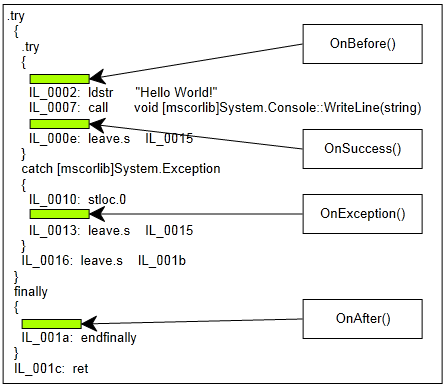
\includegraphics[scale=1.0]{MethodBoundaryOverview.PNG}
  \centering
  \caption{CIL Interception Points\label{methodboundary02}}
\end{figure}

\section{MethodAroundAspect Implementation Detail}

The MethodAroundAspect on the other hand is a much more complicated compared to the MethodBoundaryAspect.

MethodAroundAspect implements IMethodAroundAspect which has the following contract:

\begin{lstlisting}[caption={IMethodAroundAspect Interface}, label=aroundcontract]
internal interface IMethodAroundAspect : IAspect
{
	void Invoke(MethodArgs args)
}
\end{lstlisting}

When developing an aspect a Proceed() can be issued to signal a call back into the original method. The steps taken to implement MethodAroundAspect in CIL are roughly as follow:

\begin{enumerate}
	\item Create a replacement for the annotated function with exactly the same method signature.
	\item Create and store a variable pointing to the aspect.
	\item Copy all parameters from original method to the newly created replacement function.
	\item Create a variable to hold MethodArgs.
	\item Issue a call to Invoke() from the replacement function, passing in the MethodArgs variable.
	\item Handle the return value appropriately.
	\begin{enumerate}
		\item If the original method returns non void type, then put the return value back on the stack.
		\item If the original method returns void, we need to discard the return value from Invoke().
	\end{enumerate}
	\item Handle Proceed() that might be issued from inside the Invoke().
	\begin{enumerate}
		\item Load all the parameters onto the stack.
		\item Call back into the original method.
		\item Handle the return value appropriately.
	\end{enumerate}
	\item Modify all calls from original method to the replacement method.
\end{enumerate}

As figure~\ref{around_overview} shown, the actual calling of either the original or replacement method is abstracted away. This is also a testament of the saying in software engineering that "anything can be resolved by another layer of abstraction".

Another important distinction is that MethodAroundAspect currently can be applied only on the method level, and that it should be applied to one method only. This is by design because a replacement method might not be appropriate to replace more than one method. Especially if it is applied on the assembly level, all the public methods will be replaced by a single replacement method!

\section{MethodArgs Implementation Detail}

When developing an aspect, information about the target method can be accessed. This is achieved by using the MethodArgs object. During the weaving, an instance of MethodArgs is created, with all properties assembled dynamically to capture the information of the current executing method. MethodArgs is then passed as parameter into each of the aspect.

Being able to capture some information about the annotated methods will be  extremely useful in case of debugging.

A distinct instance of MethodArgs for each boundary aspects was instantiated at an early Buffalo implementation. Later on as an optimization only one instance is instantiated at the beginning of the method body and that instance is used in all the boundary aspects for a target method.

An example of how to use MethodArgs is presented in the user manual.

\chapter{Analysis}

The project hypothesized that by using Buffalo, programmers can separate the cross-cutting concerns from their applications quickly and easily. Since the concerns are encapsulated in a distinct unit of code, it also enables programmers to easily maintain the aspects and modify them as needed.

One analysis performed is to write an aspect to catch unhandled exceptions in test programs. The size of the test programs varies from comprising of 50 methods to 1,000 methods. Suppose that to manually implement the exception handling, a programmer will have to write on average 5 lines of code to catch the exception.

\begin{table}[H]
\centering
\begin{tabular}{|l|l|l|}
\hline
Programs & Lines (Traditions) & Lines (Buffalo)\\
\hline
50 & 250 & 0-1\\
500 & 2,500 & 0-1\\
1,000 & 5,000 & 0-1\\
\hline
\end{tabular}
\caption{Line counts}
\label{tab:lines_tbl}
\end{table}

If exception handling is implemented for every method by hand, more line of the same try-catch block of code will have to be written as the application adds more methods. The number of line of repetitive code would increase linearly.

Lines of code have a direct correlation to the cost of the development as it will take programmers more time. And this will also have a direct impact on application release schedule.

By using a framework like Buffalo, unhandled exception can be centralized in one aspect, and then simply apply it to every method by applying it on the assembly level. 

As a result the source code is free from the repetitive try-catch-finally blocks. The line of code we have to write is one line at most, and will stay constant even as more types and methods are added to the application. This will also give developer a peace of mind that every method will be handled automatically.

One can argue that since unhandled exceptions will bubble up the chain, a developer can simply catch them in the main method, and this would have achieved similar effect. That approach is limited in that it is very generic. When the main method catches an exception, it has no idea what the internal state of the failed method was. Using Buffalo, the internal state can be inspected by checking the MethodArgs object. 

Buffalo allows developer to quickly create aspects to solve various problems, from unhandled exception to instrumenting the application. These are just some of the scenarios where Buffalo proves to be helpful. More examples are provided in Appendix A. 

Buffalo has performed well in isolating cross-cutting concerns into single unit of code, which is easily maintained and modified.

\chapter{Conclusions}
\section{Current Status}

Buffalo currently contains two types of aspect:  MethodBoundaryAspect - where various execution points can be intercepted. MethodAroundAspect - where a method can be wrapped around or completely replaced while preserving the option to call back into the original method. MethodAroundAspect targets individual method, whereas MethodBoundaryAspect can be applied on three levels on a .NET application.

Originally MS-Build integration was planned, that when the Buffalo program was installed via the setup executable, it will modify the relevant .NET configuration files to hook BuffaloAOP.exe into MS-Build. That would trigger the weaving process from within the Visual Studio IDE when the solution is compiled. It was later found that Microsoft has dropped support for the setup project type. As a work around, instruction is provided in appendix A to manually hook into MS-Build.

Originally MethodAroundAspect was intended to be used similar to MethodBoundaryAspect, where it can be applied on three levels. However it was later determined that since the CIL instruction of the actual aspect will also have to be modified, it really does not make sense for it to be applied to more than one method, as it would introduce conflicting changes.

MethodAroundAspect improvement remains to be determined.

\section{Future Work}

There are couple areas where Buffalo can be improved upon. Usability wise, currently there is no automatic setup program that installs Buffalo onto user’s computer. There is also no automatic integration into MS-Build System. Some manual steps are still needed in order to provide a more seamless experience.

Functionality wise, when Buffalo performs post compilation weaving it starts fresh each time; it would be interesting to see how incremental weaving can be done here. Another useful functionality is to be able to apply aspects by matching a set of methods.

\section{Lessons Learned}

A framework such as Buffalo mitigates the problem of cross-cutting concerns. Still, to efficiently tackle the root of the problem, compiler vendors have to actively embrace the AOP concept and provide native support in their programming languages.

Developers also have to understand such problems and what solutions are available to better educate themselves.

Only when the concept is widely understood and supported by both developers and vendors can there hope to begin alleviating such problems.


%%%%%%%%%%%%%%%%%%%%%%%%%%%%%%%%%%%%%%%%%%%%%%%%%%%%%%%%%%%%%%%%%%%%%%%%%%%%%%%

%%%%%%%%%%%%%%%%%%%%%%%%%%%%%%%%%%%%%%%%%%%%%%%%%%%%%%%%%%%%%%%%%%%%%%%%%%%%%%%
%\bibliographystyle{plain}
\bibliographystyle{unsrt}
% Single space the bibliography to save space.
\begin{singlespace}
\bibliography{CapstoneBib}
\end{singlespace}
%%%%%%%%%%%%%%%%%%%%%%%%%%%%%%%%%%%%%%%%%%%%%%%%%%%%%%%%%%%%%%%%%%%%%%%%%%%%%%%

%%%%%%%%%%%%%%%%%%%%%%%%%%%%%%%%%%%%%%%%%%%%%%%%%%%%%%%%%%%%%%%%%%%%%%%%%%%%%%%
% The appendices are (of course) optional.
\appendix
%\chapter{UML Diagrams}

This is an optional appendix and can be eliminated if you don't have anything 
to share here.


%\chapter{Code Listing}

Buffalo is a fairly compact framework for the current functionalities. The full source code is around 1,200 lines, which is fully included here. With optimization it could probably be reduced even more. Note the short listing entitled "buffalo/BuffaloAOP/Program.cs" at the end is the entired BuffaloAOP.exe program that kicks off the weaving.

\vspace{5mm}
\begin{lstlisting}[caption={../buffalo/MethodAroundAspect.cs}, label=../buffalo/MethodAroundAspect.cs, frame=tb, basicstyle=\scriptsize]using Buffalo.Interfaces;

namespace Buffalo
{
    public abstract class MethodAroundAspect : AspectBase, IMethodAroundAspect
    {
        public virtual object Invoke(MethodArgs args) { return null; }
    }
}
\end{lstlisting}

\begin{lstlisting}[caption={../buffalo/MethodArgs.cs}, label=../buffalo/MethodArgs.cs, frame=tb, basicstyle=\scriptsize]using System;
using System.Collections.Generic;

namespace Buffalo
{
    public sealed class MethodArgs
    {
        private string name;
        private string fullName;
        private string returnTypeStr;
        private string parameterStr;
        private List<Parameter> parameters;
        private object[] parameterArray;
        private Exception exception;
        private Object instance;

        public MethodArgs()
        {
            this.parameters = new List<Parameter>();
        }

        public string Name
        {
            get
            {
                return this.name;
            }
        }

        public string FullName
        {
            get
            {
                return this.fullName;
            }
        }

        public Type ReturnType
        {
            get
            {
                return Type.GetType(this.returnTypeStr);
            }
        }

        public List<Parameter> Parameters
        {
            get { return this.parameters; }
        }

        public Exception Exception
        {
            get { return this.exception; }
        }

        public object Instance
        {
            get { return this.instance; }
        }

        public object[] ParameterArray
        {
            get { return this.parameterArray; }
        }

        public void SetProperties(string name,
            string fullname,
            string returnTypeStr,
            string parameterStr,
            object[] parameterArray,
            object instance = null)
        {
            this.name = name;
            this.fullName = fullname;
            this.returnTypeStr = returnTypeStr;
            this.parameterStr = parameterStr;
            this.parameterArray = parameterArray;
            this.instance = instance;

            var splits = this.parameterStr.Split(new char[] { '|' }, StringSplitOptions.RemoveEmptyEntries);
            foreach (var split in splits)
            {
                var p = split.Split(new char[] { ':' }, StringSplitOptions.RemoveEmptyEntries);
                this.parameters.Add(new Parameter { Name = p[0], Type = Type.GetType(p[1]) });
            }

            for (int i = 0; i < this.Parameters.Count; ++i)
            {
                this.Parameters[i].Value = this.parameterArray[i];
            }
        }

        public void SetException(Exception exception)
        {
            this.exception = exception;
        }

        public object Proceed()
        {
            return null;
        }
    }
}
\end{lstlisting}

\begin{lstlisting}[caption={../buffalo/Aspect.cs}, label=../buffalo/Aspect.cs, frame=tb, basicstyle=\scriptsize]using System;
using Buffalo.Common;
using Mono.Cecil;

namespace Buffalo
{
    internal class Aspect : IAspect
    {
        public Aspect()
        {
            this.AssemblyLevelStatus = Enums.Status.NotApplied;
        }

        public string Name { get; set; }

        public Enums.Status AssemblyLevelStatus { get; set; }

        public TypeDefinition TypeDefinition { get; set; }

        [Obsolete]
        public System.Type Type { get; set; }

        public Buffalo.Common.Enums.BuffaloAspect BuffaloAspect { get; set; }

        public override string ToString()
        {
            return this.Name;
        }
    }
}
\end{lstlisting}

\begin{lstlisting}[caption={../buffalo/MethodBoundaryAspect.cs}, label=../buffalo/MethodBoundaryAspect.cs, frame=tb, basicstyle=\scriptsize]using Buffalo.Interfaces;

namespace Buffalo
{
    public abstract class MethodBoundaryAspect : AspectBase, IMethodBoundaryAspect
    {
        public virtual void OnBefore(MethodArgs args) { }

        public virtual void OnAfter(MethodArgs args) { }

        public virtual void OnSuccess(MethodArgs args) { }

        public virtual void OnException(MethodArgs args) { }
    }
}
\end{lstlisting}

\begin{lstlisting}[caption={../buffalo/AspectBase.cs}, label=../buffalo/AspectBase.cs, frame=tb, basicstyle=\scriptsize]namespace Buffalo
{
    [System.AttributeUsage(System.AttributeTargets.All,
        AllowMultiple = false)]
    public abstract class AspectBase : System.Attribute
    {
        public AspectBase(bool attributeExclude = false)
        {
            this.AttributeExclude = attributeExclude;
        }

        public bool AttributeExclude { get; set; }
    }
}
\end{lstlisting}

\begin{lstlisting}[caption={../buffalo/Weaver.cs}, label=../buffalo/Weaver.cs, frame=tb, basicstyle=\scriptsize]using Buffalo.Common;
using Buffalo.Injectors;
using Buffalo.Interfaces;
using Mono.Cecil;
using Mono.Cecil.Cil;
using System;
using System.Collections.Generic;
//using Mono.Cecil.Rocks;
using System.Collections.Specialized;
using System.IO;
using System.Linq;
using Reflection = System.Reflection;

namespace Buffalo
{
    internal class Weaver
    {
        public Weaver(string assemblyPath)
        {
            ///TODO: Maybe just don't do anything if file not found
            if (!File.Exists(assemblyPath))
                throw new FileNotFoundException();

            AssemblyPath = assemblyPath;
            this.Init();
        }

        static internal string AssemblyPath { get; set; }

        static internal List<Aspect> Aspects { get; set; }

        static internal Dictionary<string, Type> UnderlyingAspectTypes { get; set; }

        internal Dictionary<MethodDefinition, List<Aspect>> EligibleMethods { get; set; }

        internal List<TypeDefinition> TypeDefinitions { get; set; }

        internal AssemblyDefinition AssemblyDefinition { get; set; }

        internal StringCollection NewMethodNames { get; set; }

        internal void Inject(string outPath)
        {
            var injectors = new List<IInjectable>();

            //apply the around aspect if necessary
            var aroundAspectExist = this.EligibleMethods.Values.Any(x => 
                x.Any(y => y.BuffaloAspect == Enums.BuffaloAspect.MethodAroundAspect));
            if (aroundAspectExist)
                injectors.Add(new MethodAroundInjector());

            //apply the boundary aspect if necessary
            var boundaryAspectExist = this.EligibleMethods.Values.Any(x =>
                x.Any(y => y.BuffaloAspect == Enums.BuffaloAspect.MethodBoundaryAspect));
            if (boundaryAspectExist)
                injectors.Add(new MethodBoundaryInjector());

            //inject
            injectors.ForEach(x => x.Inject(this.AssemblyDefinition, this.EligibleMethods));

            //write out the modified assembly
            this.AssemblyDefinition.Write(outPath);
            Console.WriteLine("DONE");
        }

        private void Init()
        {
            //initialize the variables
            Aspects = new List<Aspect>();
            NewMethodNames = new StringCollection();
            this.TypeDefinitions = new List<TypeDefinition>();
            this.EligibleMethods = new Dictionary<MethodDefinition, List<Aspect>>();
            //set the resolver in case assembly is in different directory
            var resolver = new DefaultAssemblyResolver();
            resolver.AddSearchDirectory(new FileInfo(AssemblyPath).Directory.FullName);
            var parameters = new ReaderParameters { AssemblyResolver = resolver };
            this.AssemblyDefinition = AssemblyDefinition.ReadAssembly(AssemblyPath, parameters);
            //populate the type definition first
            foreach (var m in this.AssemblyDefinition.Modules)
                m.Types.ToList().ForEach(x => this.TypeDefinitions.Add(x));
            //if aspects are defined in a different assembly?
            var typedefs = this.FindAspectTypeDefinition();
            this.TypeDefinitions = this.TypeDefinitions.Union(typedefs).ToList();
            //extract aspects from the type definitions
            this.TypeDefinitions
                .Where(x => x.BaseType != null)
                .ToList()
                .ForEach(x =>
                {
                    Buffalo.Common.Enums.BuffaloAspect? ba = null;
                    if (x.BaseType.FullName == typeof(MethodBoundaryAspect).FullName)
                        ba = Enums.BuffaloAspect.MethodBoundaryAspect;
                    else if (x.BaseType.FullName == typeof(MethodAroundAspect).FullName)
                        ba = Enums.BuffaloAspect.MethodAroundAspect;
                    if(ba.HasValue)
                        Aspects.Add(new Aspect { Name = x.FullName, TypeDefinition = x, BuffaloAspect = ba.Value });
                });
            Aspects.ForEach(x => x.AssemblyLevelStatus = this.CheckAspectStatus(this.AssemblyDefinition, x));
            //finally, get all the eligible methods for each aspect
            Aspects
                .Where(x => x.AssemblyLevelStatus != Enums.Status.Excluded)
                .ToList()
                .ForEach(x =>
                {
#if DEBUG
                    Console.WriteLine("Aspect {0}: {1}", x.Name, x.AssemblyLevelStatus.ToString());
                    Console.WriteLine("============================================");
#endif
                    this.CheckEligibleMethods(x);
                    Console.WriteLine("");
                });
        }

        private List<TypeDefinition> FindAspectTypeDefinition()
        {
            //look for aspect in this assembly, if aspect is defined in a different
            //assembly, import it here.
            var types = this.AssemblyDefinition.MainModule.Types;
            var tdefs = new List<TypeDefinition>();
            foreach (var ca in this.AssemblyDefinition.CustomAttributes)
            {
                var car = ca.AttributeType.Resolve();
                if (car.BaseType.FullName == typeof(MethodBoundaryAspect).FullName
                    || car.BaseType.FullName == typeof(MethodAroundAspect).FullName)
                {
                    tdefs.Add(car);
                }
            }

            //loop thru the custom attributes of each type, resolve them to find aspects
            foreach (var type in types)
            {
                if (type.CustomAttributes.Count == 0) continue;
                var cas = type.CustomAttributes;
                foreach (var ca in cas)
                {
                    var car = ca.AttributeType.Resolve();
                    if (car.BaseType.FullName == typeof(MethodBoundaryAspect).FullName
                        || car.BaseType.FullName == typeof(MethodAroundAspect).FullName)
                    {
                        if(!tdefs.Contains(car))
                            tdefs.Add(car);
                    }
                }
            }

            return tdefs;
        }

        private void PrintEligibleMethods()
        {
            foreach (var de in this.EligibleMethods)
            {
                Console.WriteLine(de.Key.FullName);
                foreach (var a in de.Value)
                    Console.WriteLine("\t" + a.Name);
            }
        }

        private void CheckEligibleMethods(Aspect aspect)
        {
            foreach (var t in this.TypeDefinitions.Where(x => !x.Name.Equals("<Module>")
                && (x.BaseType == null || (x.BaseType.FullName != typeof(MethodBoundaryAspect).FullName
                    && x.BaseType.FullName != typeof(MethodAroundAspect).FullName))))
            {
                var status = this.CheckAspectStatus(t, aspect);
#if DEBUG
                Console.WriteLine("\t{0}: {1}", t.Name, status.ToString());
#endif
                if (status == Enums.Status.Excluded)
                    continue;

                var mths = this.GetMethodDefinitions(t, status, aspect);
                mths.ForEach(x =>
                {
                    if (!this.EligibleMethods.ContainsKey(x))
                    {
                        this.EligibleMethods.Add(x, new List<Aspect>() { aspect });
                    }
                    else
                    {
                        var aspects = this.EligibleMethods[x];
                        aspects.Add(aspect);
                    }
                });
            }
        }

        private List<MethodDefinition> GetMethodDefinitions(TypeDefinition typeDef, Enums.Status typeStatus, Aspect aspect)
        {
            var list = new List<MethodDefinition>();
            foreach (var method in typeDef.Methods)
            {
                var status = this.CheckAspectStatus(method, aspect);
                if (status == Enums.Status.Applied)
                {
                    list.Add(method);
                }
                else
                {
                    if (typeStatus == Enums.Status.Applied && status != Enums.Status.Excluded)
                    {
                        status = Enums.Status.Applied;
                        list.Add(method);
                    }
                }
#if DEBUG
                Console.WriteLine("\t\t{0}: {1}", method.Name, status.ToString());
#endif
            }

            return list;
        }

        /// <summary>
        /// A TypeDefinition and MethodDefinition both implement the
        /// ICustomAttributeProvider interface, so it can be used here
        /// to determined if a method is marked as exclude or not.
        /// </summary>
        private Enums.Status CheckAspectStatus(ICustomAttributeProvider def, Aspect aspect)
        {
            Enums.Status status = aspect.AssemblyLevelStatus;

            bool attrFound = false;
            for (int i = 0; i < def.CustomAttributes.Count; ++i)
            {
                if (def.CustomAttributes[i].AttributeType.FullName.Equals("System.Runtime.CompilerServices.CompilerGeneratedAttribute"))
                {
                    status = Enums.Status.Excluded;
                    break;
                }

                if (aspect.TypeDefinition != null
                    && (aspect.BuffaloAspect == Enums.BuffaloAspect.MethodBoundaryAspect
                    || aspect.BuffaloAspect == Enums.BuffaloAspect.MethodAroundAspect))
                {
                    attrFound = true;
                    if (def.CustomAttributes[i].Properties.Count == 0)
                    {
                        status = Enums.Status.Applied;
                    }
                    else
                    {
                        var exclude = def.CustomAttributes[i].Properties.FirstOrDefault(x => x.Name == "AttributeExclude");
                        if (exclude.Argument.Value != null && (bool)exclude.Argument.Value == true)
                        {
                            status = Enums.Status.Excluded;
                            def.CustomAttributes.RemoveAt(i);
                        }
                    }
                }
            }

            if (!attrFound && aspect.AssemblyLevelStatus == Enums.Status.Applied)
            {
                //this aspect is applied on the assembly level and
                //as a result the type and method might not have the
                //attributed annotated, this is to programmatically add
                //in the annotation so IL can be generated correctly.
                var ctor = aspect.TypeDefinition.Methods.First(x => x.IsConstructor);
                var ctoref = this.AssemblyDefinition.MainModule.Import(ctor);
                def.CustomAttributes.Add(new CustomAttribute(ctoref));
            }

            return status;
        }
    }
}\end{lstlisting}

\begin{lstlisting}[caption={../buffalo/Parameter.cs}, label=../buffalo/Parameter.cs, frame=tb, basicstyle=\scriptsize]using System;

namespace Buffalo
{
    public sealed class Parameter
    {
        public Type Type { get; set; }

        public string Name { get; set; }

        public object Value { get; set; }
    }
}
\end{lstlisting}

\begin{lstlisting}[caption={../buffalo/Injectors/MethodAroundInjector.cs}, label=../buffalo/Injectors/MethodAroundInjector.cs, frame=tb, basicstyle=\scriptsize]using Buffalo.Extensions;
using Buffalo.Interfaces;
using Mono.Cecil;
using Mono.Cecil.Cil;
using System;
using System.Collections.Generic;
using System.Collections.Specialized;
using System.Linq;
//using Mono.Cecil.Rocks;

namespace Buffalo.Injectors
{
    internal class MethodAroundInjector : IInjectable
    {
        AssemblyDefinition AssemblyDefinition;
        Dictionary<MethodDefinition, List<Aspect>> EligibleMethods;

        public void Inject(Mono.Cecil.AssemblyDefinition assemblyDefinition, 
            Dictionary<Mono.Cecil.MethodDefinition, List<Aspect>> eligibleMethods)
        {
            /* The around aspect is to intercept all calls to the target method, and
             * replace those calls with a completely different method. While preserving
             * the option to call back to the target method when necessary.
             */
            this.AssemblyDefinition = assemblyDefinition;
            this.EligibleMethods = eligibleMethods;
            var NewMethodNames = new StringCollection();
            var eligibleAroundMethods = this.EligibleMethods
                .Where(x => x.Value.Any(y => y.Type.BaseType == typeof(MethodAroundAspect)));
            foreach (var d in eligibleAroundMethods)
            {
                var method = d.Key;
                var aspects = d.Value;
                var il = method.Body.GetILProcessor();
                var methodType = method.DeclaringType;
                var maInstructions = new List<Instruction>();
                var aspectVarInstructions = new List<Instruction>();
                var aroundInstructions = new List<Instruction>();

                foreach (var aspect in aspects.Where(x => x.Type.BaseType == typeof(MethodAroundAspect)))
                {
                    var varTicks = System.DateTime.Now.Ticks;

                    //create a replacement for the annotated function
                    var methodName = string.Format("{0}{1}", method.Name, varTicks);
                    MethodDefinition newmethod =
                        new MethodDefinition(methodName, method.Attributes, method.ReturnType);
                    methodType.Methods.Add(newmethod);
                    NewMethodNames.Add(methodName);
                    //newmethod.Body.SimplifyMacros();
                    newmethod.Body.InitLocals = true;

                    //create aspect variable
                    var varAspectName = "asp" + varTicks;
                    var varAspect = new VariableDefinition(varAspectName, aspect.TypeDefinition);
                    newmethod.Body.Variables.Add(varAspect);
                    var varAspectIdx = newmethod.Body.Variables.Count - 1;
                    var constructorInfo = aspect.Type.GetConstructor(new Type[] { });
                    MethodReference myClassConstructor =
                        this.AssemblyDefinition.MainModule.Import(constructorInfo);
                    //store the newly created aspect variable
                    newmethod.Body.Instructions.Add(Instruction.Create(OpCodes.Newobj, myClassConstructor));
                    newmethod.Body.Instructions.Add(Instruction.Create(OpCodes.Stloc, varAspect));
                    //copy all the paramters
                    method.Parameters.ToList().ForEach(x =>
                        newmethod.Parameters.Add(new ParameterDefinition(x.Name, x.Attributes, x.ParameterType)));
                    //create a MethodArgs
                    var var = newmethod.AddMethodArgsVariable(this.AssemblyDefinition);

                    #region Calling MethodArgs.Invoke
                    newmethod.Body.Instructions.Add(Instruction.Create(OpCodes.Ldloc, varAspect));
                    newmethod.Body.Instructions.Add(Instruction.Create(OpCodes.Ldloc, var.Var));
                    var aspectInvoke = aspect.Type.GetMethod("Invoke");
                    var aspectInvokeRef = 
                        this.AssemblyDefinition.MainModule.Import(aspectInvoke, newmethod);
                    newmethod.Body.Instructions.Add(Instruction.Create(OpCodes.Callvirt, aspectInvokeRef));
                    #endregion

                    #region Handling return value
                    if (!newmethod.ReturnType.FullName.Equals("System.Void"))
                    {
                        //create an object variable to hold the return value
                        var varObj = new VariableDefinition("obj" + varTicks,
                            this.AssemblyDefinition.MainModule.Import(typeof(object)));
                        newmethod.Body.Variables.Add(varObj);
                        newmethod.Body.Instructions.Add(
                            Instruction.Create(OpCodes.Stloc, varObj));
                        newmethod.Body.Instructions.Add(
                            Instruction.Create(OpCodes.Ldloc, varObj));
                        newmethod.Body.Instructions.Add(
                            Instruction.Create(OpCodes.Unbox_Any, newmethod.ReturnType));
                    }
                    else
                    {
                        //pop the return value since it's not used?
                        newmethod.Body.Instructions.Add(
                            Instruction.Create(OpCodes.Pop));
                    }
                    #endregion

                    #region Handling Proceed()
                    var invoke = aspect.TypeDefinition.Methods.FirstOrDefault(
                        x => x.FullName.Contains("::Invoke(Buffalo.MethodArgs)"));
                    bool found = false;
                    int instIdx = 0;
                    for (; instIdx < invoke.Body.Instructions.Count; ++instIdx)
                    {
                        if (invoke.Body.Instructions[instIdx].ToString()
                            .Contains("System.Object Buffalo.MethodArgs::Proceed"))
                        {
                            found = true;
                            break;
                        }
                    }

                    if (found)
                    {
                        var invokeInstructions = new List<Instruction>();
                        //var ins = Instruction.Create(OpCodes.Call, method);
                        //invoke.Body.Instructions[instIdx] = ins;
                        invoke.Body.Instructions.RemoveAt(instIdx);
                        var startIdx = instIdx;

                        //create a var to hold the original method type instance
                        var instance = new VariableDefinition("instance" + DateTime.Now.Ticks,
                            this.AssemblyDefinition.MainModule.Import(typeof(object)));
                        invoke.Body.Variables.Add(instance);
                        invoke.Body.InitLocals = true;

                        //get the instance obj from MethodArgs
                        var getInstance = typeof(MethodArgs).GetMethod("get_Instance");
                        var getInstanceRef = this.AssemblyDefinition.MainModule.Import(getInstance);
                        invokeInstructions.Add(Instruction.Create(OpCodes.Callvirt, getInstanceRef));
                        invokeInstructions.Add(Instruction.Create(OpCodes.Stloc, instance));

                        //create object array to hold ParameterArray
                        var objType = this.AssemblyDefinition.MainModule.Import(typeof(object));
                        var objArray = new ArrayType(objType);
                        var varArray = new VariableDefinition("va" + DateTime.Now.Ticks,
                            (TypeReference)objArray);
                        invoke.Body.Variables.Add(varArray);
                        //invokeInstructions.Add(Instruction.Create(OpCodes.Ldc_I4, method.Parameters.Count));
                        //invokeInstructions.Add(Instruction.Create(OpCodes.Newarr, objType));
                        var getParameterArray = typeof(MethodArgs).GetMethod("get_ParameterArray");
                        var getParameterArrayRef = this.AssemblyDefinition.MainModule.Import(getParameterArray);
                        invokeInstructions.Add(Instruction.Create(OpCodes.Ldarg_1));
                        invokeInstructions.Add(Instruction.Create(OpCodes.Callvirt, getParameterArrayRef));
                        invokeInstructions.Add(Instruction.Create(OpCodes.Stloc, varArray));

                        //modify the Invoke() instruction to make a call to the original method
                        invokeInstructions.Add(Instruction.Create(OpCodes.Ldloc, instance));
                        invokeInstructions.Add(Instruction.Create(OpCodes.Unbox_Any, method.DeclaringType));
                        if (method.Parameters.Count > 0)
                        {
                            for (int i = 0; i < method.Parameters.Count; ++i)
                            {
                                invokeInstructions.Add(Instruction.Create(OpCodes.Ldloc, varArray));
                                invokeInstructions.Add(il.Create(OpCodes.Ldc_I4, i));
                                invokeInstructions.Add(il.Create(OpCodes.Ldelem_Ref));
                                invokeInstructions.Add(Instruction.Create(OpCodes.Unbox_Any, method.Parameters[i].ParameterType));
                            }
                        }

                        //make the call
                        invokeInstructions.Add(Instruction.Create(OpCodes.Callvirt, method));

                        #region Handling return value
                        if (!method.ReturnType.FullName.Equals("System.Void"))
                        {
                            //create an object variable to hold the return value
                            var varObj = new VariableDefinition("obj" + DateTime.Now.Ticks,
                                this.AssemblyDefinition.MainModule.Import(typeof(object)));
                            invoke.Body.Variables.Add(varObj);
                            invokeInstructions.Add(
                                Instruction.Create(OpCodes.Box, method.ReturnType));
                        }
                        else
                        {
                            //method is suppose to return void, but since
                            //previously it calls Proceed() which returns object type,
                            //we need to handle that.
                            invoke.Body.Instructions[instIdx] = Instruction.Create(OpCodes.Nop);
                        }
                        #endregion

                        //write out the instruction
                        invokeInstructions.ForEach(
                            x => invoke.Body.Instructions.Insert(startIdx++, x));
                    }
                    #endregion

                    #region Modify all calls from origin to the generated method
                    foreach (var type in this.AssemblyDefinition.MainModule.Types
                        .Where(x => x.BaseType == null || !x.BaseType.FullName.Equals("Buffalo.MethodAroundAspect")))
                    {
                        var methods = type.Methods.Where(x => !NewMethodNames.Contains(x.Name));
                        foreach (var m in methods)
                        {
                            for (int j = 0; j < m.Body.Instructions.Count; ++j)
                            {
                                if (m.Body.Instructions[j].ToString().Contains(method.FullName))
                                {
                                    m.Body.Instructions[j].Operand = newmethod;
                                    //MethodArgs.Invoke returns an object, need to unbox it here to the original type
                                    //However, unboxing is needed only if the original method has a return type
                                    //other than void
                                    if (!newmethod.ReturnType.FullName.Equals("System.Void"))
                                    {
                                        //var unbox = Instruction.Create(OpCodes.Unbox_Any, newmethod.ReturnType);
                                        //var il2 = m.Body.GetILProcessor();
                                        //il2.InsertAfter(m.Body.Instructions[j], unbox);
                                    }
                                }
                            }
                        }
                    }
                    #endregion

                    newmethod.Body.Instructions.Add(Instruction.Create(OpCodes.Ret));
                    //newmethod.Body.OptimizeMacros();
                }
            }
        }
    }
}
\end{lstlisting}

\begin{lstlisting}[caption={../buffalo/Injectors/MethodBoundaryInjector.cs}, label=../buffalo/Injectors/MethodBoundaryInjector.cs, frame=tb, basicstyle=\scriptsize]using Buffalo.Common;
using Buffalo.Extensions;
using Buffalo.Interfaces;
using Mono.Cecil;
using Mono.Cecil.Cil;
using System;
using System.Collections.Generic;
using System.Linq;
//using Mono.Cecil.Rocks;

namespace Buffalo.Injectors
{
    internal class MethodBoundaryInjector : IInjectable
    {
        AssemblyDefinition AssemblyDefinition;
        Dictionary<MethodDefinition, List<Aspect>> EligibleMethods;

        public void Inject(AssemblyDefinition assemblyDefinition, Dictionary<MethodDefinition, List<Aspect>> eligibleMethods)
        {
            this.AssemblyDefinition = assemblyDefinition;
            this.EligibleMethods = eligibleMethods;

            var ems = this.EligibleMethods.ToList();
            var eligibleBoundaryMethods = ems.Where(x => x.Value.Any(y =>
                y.BuffaloAspect == Enums.BuffaloAspect.MethodBoundaryAspect));
            foreach (var d in eligibleBoundaryMethods)
            {
                var method = d.Key;
                if (method.Body == null)
                {
#if DEBUG
                    Console.WriteLine(string.Format("{0} has empty body, skipping", method.FullName));
#endif
                    continue;
                }
                var aspects = d.Value;
                var il = method.Body.GetILProcessor();
                var voidType = method.ReturnType.FullName.Equals("System.Void");
                var ret = il.Create(OpCodes.Ret);

                var maInstructions = new List<Instruction>();
                var aspectVarInstructions = new List<Instruction>();
                var beforeInstructions = new List<Instruction>();
                var successInstructions = new List<Instruction>();
                var exceptionInstructions = new List<Instruction>();
                var afterInstructions = new List<Instruction>();

                //method.Body.SimplifyMacros();
                #region Method detail
                //create a MethodArgs
                var var = method.AddMethodArgsVariable(this.AssemblyDefinition);
                #endregion

                #region Before, Success, Exception, After
                var varExpTypeRef = this.AssemblyDefinition.MainModule.Import(typeof(System.Exception));
                for (int i = 0; i < aspects.Count; ++i)
                {
                    #region Create an aspect variable
                    var varAspectName = "asp" + System.DateTime.Now.Ticks;
                    var varAspect = new VariableDefinition(varAspectName, aspects[i].TypeDefinition);
                    method.Body.Variables.Add(varAspect);
                    var varAspectIdx = method.Body.Variables.Count - 1;
                    //call ctor
                    var ctor = aspects[i].TypeDefinition.Methods.First(x => x.IsConstructor);
                    aspectVarInstructions.Add(Instruction.Create(OpCodes.Newobj, ctor));
                    aspectVarInstructions.Add(Instruction.Create(OpCodes.Stloc, varAspect));
                    #endregion

                    #region Before, success, exception
                    var before = method.FindMethodReference(aspects[i], Enums.AspectType.OnBefore);
                    if (before != null)
                    {

                        beforeInstructions.Add(Instruction.Create(OpCodes.Ldloc, varAspect));
                        beforeInstructions.Add(Instruction.Create(OpCodes.Ldloc, var.Var));
                        var aspectBefore = aspects[i].TypeDefinition.Methods.FirstOrDefault(
                            x => x.Name == Enums.AspectType.OnBefore.ToString());
                        beforeInstructions.Add(Instruction.Create(OpCodes.Callvirt, aspectBefore));
                    }

                    var success = method.FindMethodReference(aspects[i], Enums.AspectType.OnSuccess);
                    if (success != null)
                    {
                        successInstructions.Add(Instruction.Create(OpCodes.Ldloc, varAspect));
                        successInstructions.Add(Instruction.Create(OpCodes.Ldloc, var.Var));
                        var aspectSuccess = aspects[i].TypeDefinition.Methods.FirstOrDefault(
                            x => x.Name == Enums.AspectType.OnSuccess.ToString());
                        successInstructions.Add(Instruction.Create(OpCodes.Callvirt, aspectSuccess));
                    }

                    var exception = method.FindMethodReference(aspects[i], Enums.AspectType.OnException);
                    if (exception != null)
                    {
                        var expName = "exp" + System.DateTime.Now.Ticks;
                        var varExp = new VariableDefinition(expName, varExpTypeRef);
                        method.Body.Variables.Add(varExp);
                        exceptionInstructions.Add(Instruction.Create(OpCodes.Stloc, varExp));
                        exceptionInstructions.Add(Instruction.Create(OpCodes.Ldloc, var.Var));
                        exceptionInstructions.Add(Instruction.Create(OpCodes.Ldloc, varExp));
                        var maSetException = typeof(MethodArgs).GetMethod("SetException");
                        var maSetExceptionRef = this.AssemblyDefinition.MainModule.Import(maSetException, method);
                        exceptionInstructions.Add(Instruction.Create(OpCodes.Callvirt, maSetExceptionRef));

                        exceptionInstructions.Add(Instruction.Create(OpCodes.Ldloc, varAspect));
                        exceptionInstructions.Add(Instruction.Create(OpCodes.Ldloc, var.Var));
                        var aspectException = aspects[i].TypeDefinition.Methods.FirstOrDefault(
                            x => x.Name == Enums.AspectType.OnException.ToString());
                        exceptionInstructions.Add(Instruction.Create(OpCodes.Callvirt, aspectException));
                    }

                    var after = method.FindMethodReference(aspects[i], Enums.AspectType.OnAfter);
                    if (after != null)
                    {
                        afterInstructions.Add(Instruction.Create(OpCodes.Ldloc, varAspect));
                        afterInstructions.Add(Instruction.Create(OpCodes.Ldloc, var.Var));
                        var aspectAfter = aspects[i].TypeDefinition.Methods.FirstOrDefault(
                            x => x.Name == Enums.AspectType.OnAfter.ToString());
                        afterInstructions.Add(Instruction.Create(OpCodes.Callvirt, aspectAfter));
                    }
                    #endregion
                }

                int varIdx = var.VarIdx;
                //maInstructions.ForEach(x => method.Body.Instructions.Insert(varIdx++, x));
                aspectVarInstructions.ForEach(x => method.Body.Instructions.Insert(varIdx++, x));

                int beforeIdx = varIdx;
                //perform this only if user overrides Before() in the aspect
                if (beforeInstructions.Count > 0)
                {
                    beforeInstructions.ForEach(x => method.Body.Instructions.Insert(beforeIdx++, x));
                }

                /* the last instruction after success should jump to return, or 3 instruction before
                 * return if return type is not void, or as an optimization, maybe we can even skip
                 * directly to last() - 2?
                 */
                var successRet = voidType ? method.Body.Instructions.Last() :
                    method.Body.Instructions[method.Body.Instructions.Count - 3];
                Instruction successLeave = il.Create(OpCodes.Leave, successRet);
                ///TODO: need to double check the format of the MSIL return
                ///br.s, ldloc, ret when return type is not void, thereby decrement by 3
                int successIdx = voidType ? method.Body.Instructions.Count - 1 : method.Body.Instructions.Count - 3;
                //perform this only if user overrides Success() in the aspect
                successInstructions.Add(successLeave);
                if (successInstructions.Count > 0)
                {
                    successInstructions.ForEach(x => method.Body.Instructions.Insert(successIdx++, x));
                }

                int exceptionIdx = voidType ? method.Body.Instructions.Count - 1 : method.Body.Instructions.Count - 3;
                int exceptionIdxConst = exceptionIdx;
                var exceptionRet = voidType ? method.Body.Instructions.Last() :
                    method.Body.Instructions[method.Body.Instructions.Count - 3];
                Instruction exceptionLeave = il.Create(OpCodes.Leave, exceptionRet);
                //perform this only if user overrides Exception() in the aspect
                if (exceptionInstructions.Count > 0)
                {
                    exceptionInstructions.Add(exceptionLeave);
                    exceptionInstructions.ForEach(x => method.Body.Instructions.Insert(exceptionIdx++, x));
                }

                var afterRet = voidType ? method.Body.Instructions.Last() :
                    method.Body.Instructions[method.Body.Instructions.Count - 3];
                var endfinally = il.Create(OpCodes.Endfinally);
                int afterIdx = voidType ? method.Body.Instructions.Count - 1 : method.Body.Instructions.Count - 3;
                int afterIdxConst = afterIdx;
                //perform this only if user overrides After() in the aspect
                if (afterInstructions.Count > 0)
                {
                    afterInstructions.Add(endfinally);
                    afterInstructions.ForEach(x => method.Body.Instructions.Insert(afterIdx++, x));
                }

                #endregion

                #region Catch..Finally..
                //add the catch block only if user overrides Exception() in the aspect
                if (exceptionInstructions.Count > 0)
                {
                    var catchHandler = new ExceptionHandler(ExceptionHandlerType.Catch)
                    {
                        TryStart = method.Body.Instructions[varIdx],
                        TryEnd = successLeave.Next,
                        HandlerStart = method.Body.Instructions[exceptionIdxConst],
                        HandlerEnd = exceptionLeave.Next,
                        CatchType = varExpTypeRef,
                    };
                    method.Body.ExceptionHandlers.Add(catchHandler);
                }

                //add the finally block only if user overrides After() in the aspect
                if (afterInstructions.Count > 0)
                {
                    var finallyHandler = new ExceptionHandler(ExceptionHandlerType.Finally)
                    {
                        TryStart = method.Body.Instructions[varIdx],
                        TryEnd = method.Body.Instructions[afterIdxConst],
                        HandlerStart = method.Body.Instructions[afterIdxConst],
                        HandlerEnd = afterRet,
                        CatchType = null,
                    };
                    method.Body.ExceptionHandlers.Add(finallyHandler);
                }
                #endregion
                //method.Body.OptimizeMacros();
            }
        }
    }
}
\end{lstlisting}

\begin{lstlisting}[caption={../buffalo/Properties/AssemblyInfo.cs}, label=../buffalo/Properties/AssemblyInfo.cs, frame=tb, basicstyle=\scriptsize]using System.Reflection;
using System.Runtime.CompilerServices;
using System.Runtime.InteropServices;

// General Information about an assembly is controlled through the following 
// set of attributes. Change these attribute values to modify the information
// associated with an assembly.
[assembly: AssemblyTitle("Buffalo")]
[assembly: AssemblyDescription("")]
[assembly: AssemblyConfiguration("")]
[assembly: AssemblyCompany("Microsoft")]
[assembly: AssemblyProduct("Buffalo")]
[assembly: AssemblyCopyright("Copyright © Microsoft 2012")]
[assembly: AssemblyTrademark("")]
[assembly: AssemblyCulture("")]

// Setting ComVisible to false makes the types in this assembly not visible 
// to COM components.  If you need to access a type in this assembly from 
// COM, set the ComVisible attribute to true on that type.
[assembly: ComVisible(false)]

// The following GUID is for the ID of the typelib if this project is exposed to COM
[assembly: Guid("625c6e79-7034-48cf-8689-b9e44f3bf96d")]

// Version information for an assembly consists of the following four values:
//
//      Major Version
//      Minor Version 
//      Build Number
//      Revision
//
// You can specify all the values or you can default the Build and Revision Numbers 
// by using the '*' as shown below:
// [assembly: AssemblyVersion("1.0.*")]
[assembly: AssemblyVersion("0.1.0.0")]
[assembly: AssemblyFileVersion("0.1.0.0")]
[assembly: InternalsVisibleTo("BuffaloAOP")]\end{lstlisting}

\begin{lstlisting}[caption={../buffalo/Common/BeginEndMarker.cs}, label=../buffalo/Common/BeginEndMarker.cs, frame=tb, basicstyle=\scriptsize]using Mono.Cecil.Cil;

namespace Buffalo.Common
{
    internal struct BeginEndMarker
    {
        public int BeginIndex { get; set; }
        public int EndIndex { get; set; }
    }
}
\end{lstlisting}

\begin{lstlisting}[caption={../buffalo/Common/Enums.cs}, label=../buffalo/Common/Enums.cs, frame=tb, basicstyle=\scriptsize]namespace Buffalo.Common
{
    internal class Enums
    {
        internal enum Status
        {
            Applied,
            NotApplied,
            Excluded
        }

        internal enum AspectType
        {
            OnBefore,
            OnAfter,
            OnSuccess,
            OnException,
            Invoke
        }

        internal enum BuffaloAspect
        {
            MethodBoundaryAspect,
            MethodAroundAspect
        }
    }
}
\end{lstlisting}

\begin{lstlisting}[caption={../buffalo/Extensions/Extensions.cs}, label=../buffalo/Extensions/Extensions.cs, frame=tb, basicstyle=\scriptsize]using Buffalo.Common;
using Mono.Cecil;
using Mono.Cecil.Cil;
using System;
using System.Collections.Generic;
using System.Linq;
using System.Text;

namespace Buffalo.Extensions
{
    internal static class Extensions
    {
        internal static MethodReference FindMethodReference(this MethodDefinition method, Aspect aspect, Enums.AspectType name)
        {
            return aspect
                .TypeDefinition
                .Methods
                .FirstOrDefault(x => x.Name.Equals(name.ToString()));
        }

        internal static VariableResult AddMethodArgsVariable(this MethodDefinition method,
            AssemblyDefinition assemblyDef)
        {
            var var = new VariableResult();
            var instructions = new List<Instruction>();
            method.Body.InitLocals = true;
            var il = method.Body.GetILProcessor();
            var isValueType = false;
            
            //create var to hold parameter count
            var pcVar = new VariableDefinition("pc" + DateTime.Now.Ticks,
                assemblyDef.MainModule.Import(typeof(int)));
            method.Body.Variables.Add(pcVar);
            instructions.Add(Instruction.Create(OpCodes.Ldc_I4, method.Parameters.Count));
            instructions.Add(Instruction.Create(OpCodes.Stloc, pcVar));

            //create an object array to hold the parameter values
            var objType = assemblyDef.MainModule.Import(typeof(object));
            var objArray = new ArrayType(objType);
            var varArray = new VariableDefinition("va" + DateTime.Now.Ticks,
                (TypeReference)objArray);
            method.Body.Variables.Add(varArray);
            instructions.Add(Instruction.Create(OpCodes.Ldloc, pcVar));
            instructions.Add(Instruction.Create(OpCodes.Newarr, objType));
            instructions.Add(Instruction.Create(OpCodes.Stloc, varArray));

            #region Handle paramters
            //loop thru the parameters, extract the values and 
            //store them in MethodArgs.ParameterArray
            TypeSpecification typeSpec = null;
            for (int i = 0; i < method.Parameters.Count; ++i )
            {
                var metaType = method.Parameters[i].ParameterType.MetadataType;
                if (metaType == MetadataType.UIntPtr
                    || metaType == MetadataType.FunctionPointer
                    || metaType == MetadataType.IntPtr
                    || metaType == MetadataType.Pointer)
                    continue;

                instructions.Add(Instruction.Create(OpCodes.Ldloc, varArray));
                instructions.Add(Instruction.Create(OpCodes.Ldc_I4, i));
                if (method.IsStatic)
                    instructions.Add(il.Create(OpCodes.Ldarg, i));
                else
                    instructions.Add(il.Create(OpCodes.Ldarg, i + 1));

                isValueType = false;
                var pType = method.Parameters[i].ParameterType;
                if (pType.IsByReference)
                {
                    typeSpec = pType as TypeSpecification;
                    if (typeSpec != null)
                    {
                        switch (typeSpec.ElementType.MetadataType)
                        {
                            case MetadataType.Boolean:
                            case MetadataType.SByte:
                                instructions.Add(Instruction.Create(OpCodes.Ldind_I1)); 
                                isValueType = true;
                                break;
                            case MetadataType.Int16:
                                instructions.Add(Instruction.Create(OpCodes.Ldind_I2)); 
                                isValueType = true;
                                break;
                            case MetadataType.Int32:
                                instructions.Add(Instruction.Create(OpCodes.Ldind_I4)); 
                                isValueType = true;
                                break;
                            case MetadataType.Int64:
                            case MetadataType.UInt64:
                                instructions.Add(Instruction.Create(OpCodes.Ldind_I8)); 
                                isValueType = true;
                                break;
                            case MetadataType.Byte:
                                instructions.Add(Instruction.Create(OpCodes.Ldind_U1)); 
                                isValueType = true;
                                break;
                            case MetadataType.UInt16:
                                instructions.Add(Instruction.Create(OpCodes.Ldind_U2)); 
                                isValueType = true;
                                break;
                            case MetadataType.UInt32:
                                instructions.Add(Instruction.Create(OpCodes.Ldind_U4)); 
                                isValueType = true;
                                break;
                            case MetadataType.Single:
                                instructions.Add(Instruction.Create(OpCodes.Ldind_R4));
                                isValueType = true;
                                break;
                            case MetadataType.Double:
                                instructions.Add(Instruction.Create(OpCodes.Ldind_R8));
                                isValueType = true;
                                break;
                            case MetadataType.IntPtr:
                            case MetadataType.UIntPtr:
                                instructions.Add(Instruction.Create(OpCodes.Ldind_I));
                                isValueType = true;
                                break;
                            default:
                                if (typeSpec.ElementType.IsValueType)
                                {
                                    instructions.Add(Instruction.Create(OpCodes.Ldobj, typeSpec.ElementType));
                                    isValueType = true;
                                }
                                else
                                {
                                    instructions.Add(Instruction.Create(OpCodes.Ldind_Ref));
                                    isValueType = false;
                                }
                                break;
                        }
                    }
                }

                if (pType.IsValueType || isValueType)
                {
                    if(isValueType)
                        instructions.Add(Instruction.Create(OpCodes.Box, typeSpec.ElementType));
                    else
                        instructions.Add(Instruction.Create(OpCodes.Box, pType));
                }

                instructions.Add(Instruction.Create(OpCodes.Stelem_Ref));
            }
            #endregion

            StringBuilder sb = new StringBuilder();
            method.Parameters.ToList()
                .ForEach(x =>
                {
                    sb.Append(string.Format("{0}:{1}|", x.Name, x.ParameterType.FullName));
                });

            var maType = typeof(MethodArgs);
            var maName = "ma" + DateTime.Now.Ticks;
            var maSetProperties = maType.GetMethod("SetProperties");
            var varMa = new VariableDefinition(maName, assemblyDef.MainModule.Import(maType));
            method.Body.Variables.Add(varMa);
            var vaMaIdx = method.Body.Variables.Count - 1;
            var maCtr = maType.GetConstructor(new Type[] { });
            MethodReference maCtrRef = assemblyDef.MainModule.Import(maCtr);
            instructions.Add(Instruction.Create(OpCodes.Newobj, maCtrRef));
            instructions.Add(Instruction.Create(OpCodes.Stloc, varMa));
            instructions.Add(Instruction.Create(OpCodes.Ldloc, varMa));
            instructions.Add(Instruction.Create(OpCodes.Ldstr, method.Name));
            instructions.Add(Instruction.Create(OpCodes.Ldstr, method.FullName));
            instructions.Add(Instruction.Create(OpCodes.Ldstr, method.ReturnType.FullName));
            instructions.Add(Instruction.Create(OpCodes.Ldstr, sb.ToString()));
            instructions.Add(Instruction.Create(OpCodes.Ldloc, varArray));
            if (method.IsStatic)
                instructions.Add(Instruction.Create(OpCodes.Ldnull));
            else
                instructions.Add(Instruction.Create(OpCodes.Ldarg_0));

            var maSetPropertiesRef = assemblyDef.MainModule.Import(maSetProperties, method);
            instructions.Add(Instruction.Create(OpCodes.Callvirt, maSetPropertiesRef));

            int idx = 0;
            instructions.ForEach(x => method.Body.Instructions.Insert(idx++, x));

            var.Var = varMa;
            var.ParamArray = varArray;
            var.VarIdx = idx;
            return var;
        }
    }

    internal class VariableResult
    {
        public VariableDefinition Var { get; set; }
        public VariableDefinition ParamArray { get; set; }
        public int VarIdx { get; set; }
    }
}
\end{lstlisting}

\begin{lstlisting}[caption={../buffalo/Interfaces/IMethodAroundAspect.cs}, label=../buffalo/Interfaces/IMethodAroundAspect.cs, frame=tb, basicstyle=\scriptsize]namespace Buffalo.Interfaces
{
    internal interface IMethodAroundAspect : IAspect
    {
        object Invoke(MethodArgs args);
    }
}
\end{lstlisting}

\begin{lstlisting}[caption={../buffalo/Interfaces/IInjectable.cs}, label=../buffalo/Interfaces/IInjectable.cs, frame=tb, basicstyle=\scriptsize]using System.Collections.Generic;
using Mono.Cecil;

namespace Buffalo.Interfaces
{
    internal interface IInjectable
    {
        void Inject(AssemblyDefinition assemblyDefinition, Dictionary<MethodDefinition, List<Aspect>> eligibleMethods);
    }
}
\end{lstlisting}

\begin{lstlisting}[caption={../buffalo/Interfaces/IMethodBoundaryAspect.cs}, label=../buffalo/Interfaces/IMethodBoundaryAspect.cs, frame=tb, basicstyle=\scriptsize]namespace Buffalo.Interfaces
{
    internal interface IMethodBoundaryAspect : IAspect
    {
        void OnBefore(MethodArgs args);
        void OnAfter(MethodArgs args);
        void OnSuccess(MethodArgs args);
        void OnException(MethodArgs args);
    }
}
\end{lstlisting}

\begin{lstlisting}[caption={../buffalo/Interfaces/IAspect.cs}, label=../buffalo/Interfaces/IAspect.cs, frame=tb, basicstyle=\scriptsize]namespace Buffalo
{
    /// <summary>
    /// This is the base aspect interface
    /// </summary>
    internal interface IAspect
    {
    }
}
\end{lstlisting}

\begin{lstlisting}[caption={../../buffalo/BuffaloAOP/Program.cs}, label=../../buffalo/BuffaloAOP/Program.cs, frame=tb, basicstyle=\scriptsize]using System;
using System.Collections.Generic;
using System.Linq;
using System.Text;
using System.Reflection;
using Buffalo;

namespace BuffaloAOP
{
    class Program
    {
        static string path;
        static void Main(string[] args)
        {
            if (args == null || args.Count() == 0)
            {
                Console.WriteLine("USAGE: BuffaloAOP.exe <assembly_path>");
                Environment.Exit(1);
            }

            path = args[0];
            path = @"C:\Users\wliao\Documents\Visual Studio 2012\Projects\Tests\BuffaloTest\BuffaloTest\bin\Debug\Shared.dll";
            string outpath = path.Replace(".exe", "_modified.exe").Replace(".dll", "_modified.dll");
            new Weaver(path).Inject(outpath);
            //Console.Read();
        }
    }
}
\end{lstlisting}



\chapter{User Manual}

It is easy to get start using Buffalo. I assume you are reasonably familiar with the Visual Studio IDE and the general layout of a VS solution. I also assume you know how to compile a solution and where to find the compiled assembly. Buffalo is developed in VS2012, it is recommended you have the same version of the IDE installed.

\section{Compiling}
To begin, first download the full source code from https://github.com/wliao008/buffalo. Open buffalo.sln in VS2012 and compile the source code. This will produce the Buffalo.dll and BuffaloAOP.exe in their respective bin/debug folder.

For this example we will perform the weaving from a command prompt. So create a folder name under the C drive, here I will call it "Buffalo". Copy Buffalo.dll, BuffaloAOP.exe and Mono.Cecil.dll to C:\textbackslash{Buffalo}. Note this folder can be located anywhere in your system, I am just putting it on the C drive for simplicity.

Now let us create an aspect.

\section{Simple Profiler}
In this example we will create a profiler for our application. Suppose we have the following simple program.

\begin{lstlisting}[caption={Hello program}, label=helloprogram, frame=tb, basicstyle=\scriptsize]
using System;

namespace Hello
{
    class Program
    {
        static void Main(string[] args)
        {
            Hello h = new Hello();
            h.SayHello();
            h.Say("Hey Buffalo how's it going!");

            //pause the console
            Console.Read();
        }
    }

    public class Hello
    {
        public void SayHello()
        {
            Console.WriteLine("Hello World!");
        }

        public void Say(string msg)
        {
            Console.WriteLine(msg);
        }
    }
}
\end{lstlisting}

When the program runs, it will display the following output:
\begin{lstlisting}[caption={Hello program output}, label=helloout, frame=tb, basicstyle=\scriptsize]
Hello World!
Hey Buffalo how's it going!
\end{lstlisting}

And suppose that we want to monitor the program, we want to know when a method was accessed and exited. We can easily create a aspect to do such work.

\begin{lstlisting}[caption={TraceAspect}, label=traceaspect, frame=tb, basicstyle=\scriptsize]
using Buffalo;
using System;

public class TraceAspect : MethodBoundaryAspect
{
    public override void Before(MethodArgs args)
    {
        Display("ENTERING", args);
    }

    public override void After(MethodArgs args)
    {
        Display("EXITING", args);
    }

    public override void Success(MethodArgs args)
    {
        Display("SUCCESSFULLY EXECUTED", args);
    }

    public override void Exception(MethodArgs args)
    {
        Display("EXCEPTION ON", args);
    }

    void Display(string title, MethodArgs args)
    {
        Console.WriteLine("{0} {1}", title, args.FullName);
        foreach (var p in args.Parameters)
        {
            Console.WriteLine("\t{0} ({1}) = {2}", p.Name, p.Type, p.Value);
        }
    }
}
\end{lstlisting}

With the aspect defined, now we can apply this aspect on any of the three different levels. Lets apply it to the Hello class for example.
\begin{lstlisting}[caption={Apply Aspect to the Hello Class}, label=helloaspect, frame=tb, basicstyle=\scriptsize]
[TraceAspect]
public class Hello
{
	//...
}
\end{lstlisting}

Now everything is in place. We can now invoke the BuffaloAOP.exe to perform the weaving. Open a command prompt and navigate to C:\textbackslash{Buffalo}. And issue this command:

\begin{lstlisting}[caption={Invoking BuffaloAOP.exe}, label=buffalocmd, frame=tb, basicstyle=\scriptsize]
C:\Buffalo>BuffaloAOP.exe <path_to_the_hello_program_exe>
\end{lstlisting}

Replace path to the hello program exe with the actual complete path to the program assembly. Suppose the program assembly is located at C:\textbackslash{Projects}\textbackslash{Hello}\textbackslash{bin}\textbackslash{Hello.exe}, we would issue the command as follow:

\begin{lstlisting}[caption={Invoking BuffaloAOP.exe Example}, label=buffalocmd2, frame=tb, basicstyle=\scriptsize]
C:\Buffalo>BuffaloAOP.exe C:\Projects\Hello\bin\Hello.exe
\end{lstlisting}

If everything goes well BuffaloAOP.exe will perform the injection and put the final assembly in the Modified folder inside the folder of the target assembly. In this case it will be at C:\textbackslash{Projects}\textbackslash{Hello}\textbackslash{bin}\textbackslash{Modified}\textbackslash{Hello.exe}. Now when the program runs, it will display the following output:

\begin{lstlisting}[caption={TraceAspect output}, label=traceaspectout, frame=tb, basicstyle=\scriptsize]
ENTERING System.Void Hello.Program::Main(System.String[])
        args (System.String[]) = System.String[]
ENTERING System.Void Hello.Hello::.ctor()
SUCCESSFULLY EXECUTED System.Void Hello.Hello::.ctor()
EXITING System.Void Hello.Hello::.ctor()
ENTERING System.Void Hello.Hello::SayHello()
Hello World!
SUCCESSFULLY EXECUTED System.Void Hello.Hello::SayHello()
EXITING System.Void Hello.Hello::SayHello()
ENTERING System.Void Hello.Hello::Say(System.String)
        msg (System.String) = Hey Buffalo how's it going!
Hey Buffalo how's it going!
SUCCESSFULLY EXECUTED System.Void Hello.Hello::Say(System.String)
        msg (System.String) = Hey Buffalo how's it going!
EXITING System.Void Hello.Hello::Say(System.String)
        msg (System.String) = Hey Buffalo how's it going!
\end{lstlisting}

Line 7 and 12 are the original method output, the rest are the output of the various interception points. Note that line 2, 11, 14 and 16 show the parameter value passed into each method.

\section{Integrate With MS-Build System}

Buffalo can be integrated with MS-Build, so weaving can be invoked automatically when a project is compiled from the Visual Studio IDE. Note that the following instructions are just the bare minimum to get this working, a lot of bell and whistle are omitted.

MS-Build is integrated with Visual Studio IDE via configuration file. For example, a C\# project has the associated .csproj, if open in a text editor you will see a line that references a different configuration file: Microsoft.CSharp.targets. This file in term references Microsoft.Common.targets.

Each .NET version has its own Microsoft.Common.targets file. Depending on the version you are using, open up this file in a text editor. For example, for .NET 4.0, this file is located in C:\textbackslash Windows\textbackslash Microsoft.NET\textbackslash Framework\textbackslash v4.0.30319\textbackslash Microsoft.Common.targets.

Under the Compile section, around line \#2013, add the line to import the Buffalo.targets file as shown in figure~\ref{buffalo_targets}

\begin{figure}[H]
  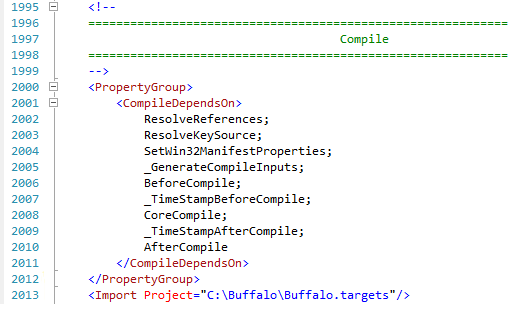
\includegraphics[scale=1.0]{CommonTarget.PNG}
  \centering
  \caption{Adding Buffalo.targets\label{buffalo_targets}}
\end{figure}

If you open Buffalo.targets in a text editor, it contains the following context:

\begin{lstlisting}[caption={Buffalo.targets}, label=buffalotargets, frame=tb, basicstyle=\scriptsize]
<Project xmlns="http://schemas.microsoft.com/developer/msbuild/2003">
  <PropertyGroup>
    <CompileDependsOn>
      $(CompileDependsOn);
      Buffalo
    </CompileDependsOn>
  </PropertyGroup>

  <Target Name="Buffalo">
    <Message Text="Hello Buffalo! @(IntermediateAssembly)"/>
    <Exec Command="&quot;C:\Buffalo\BuffaloAOP.exe&quot; &quot;@(IntermediateAssembly)&quot;"/>
  </Target>
</Project>
\end{lstlisting}

This is how Buffalo get hooked into MS-Build, what this mean is that when user compiles a project, everything defined in the CompileDependsOn property group will be performed first, then a new target named "Buffalo" will be called immediately, which will invoke the BuffaloAOP via the Exec Command. Note that for the Exec Command, a complete path to BuffaloAOP.exe must be provided, including the encoded quotation marks as shown.

Make sure to save all the changes. 

Now every time a C\# project is compiled, Buffalo will be invoked automatically to perform the weaving.

% ...
%%%%%%%%%%%%%%%%%%%%%%%%%%%%%%%%%%%%%%%%%%%%%%%%%%%%%%%%%%%%%%%%%%%%%%%%%%%%%%%
\end{document}
